\documentclass[12pt,a4paper]{article}

\usepackage[utf8]{inputenc}
\usepackage[T1]{fontenc}
\usepackage[french]{babel}
\usepackage{geometry}
\usepackage{booktabs}
\usepackage{array}
\usepackage{tabularx}
\usepackage{hyperref}
\usepackage{xcolor}
\usepackage{listings}
\usepackage{cite}
\usepackage{graphicx}
\usepackage{float}
\usepackage{parskip}

\geometry{margin=2.5cm}

\hypersetup{
    colorlinks=true,
    linkcolor=blue!60!black,
    citecolor=blue!60!black,
    urlcolor=blue!60!black
}



\title{%
    \large Projet de fin de formation — L3 Informatique et Systèmes\\[0.5em]
    \LARGE Topologie et choix architecturaux\\
}

\date{Année universitaire 2025--2026}
    



\begin{document}

\maketitle

\newpage
\tableofcontents
\newpage

% ============================================================
\section{Contexte et objectif du laboratoire}
% ============================================================

Le présent document décrit et justifie la topologie réseau et les choix
techniques du laboratoire virtualisé utilisé pour le projet
\textit{NYX}. L'objectif du laboratoire
est de simuler fidèlement l'infrastructure numérique d'une petite ou moyenne
entreprise (PME) togolaise afin de valider un moteur de corrélation d'événements
de sécurité à développer en Python.

D'après la Stratégie nationale de cybersécurité 2024--2028 de l'Agence
Nationale de la Cybersécurité du Togo (ANCy), les PME constituent une cible
prioritaire des cyberattaquants en raison de leur adoption croissante des
outils numériques et de leur faible maturité en sécurité \cite{ancy_strategie}.
Le rapport Africa Cyberthreat Assessment 2025 d'INTERPOL identifie le phishing,
la compromission de messagerie professionnelle (BEC) et l'exfiltration de
données financières comme les menaces dominantes en Afrique de l'Ouest
\cite{interpol2025}.

Le laboratoire est entièrement virtualisé sur deux machines hôtes physiques
(16~Go de RAM chacune) sous Fedora~44 et Pop~OS, en utilisant
KVM/QEMU comme hyperviseur.

% ============================================================
\section{Principes fondateurs de la topologie}
% ============================================================

Trois principes ont guidé la conception de la topologie.

\textbf{Fidélité contextuelle.} Chaque composant du laboratoire correspond
à un équipement réellement utilisé dans les PME de la région. L'objectif
n'est pas de simuler un environnement générique, mais de reproduire les
choix technologiques concrets des entreprises togolaises à budget contraint.

\textbf{Visibilité réseau complète.} Tout le trafic entre machines du laboratoire
doit traverser le pare-feu afin d'être journalisé. Cette contrainte impose
qu'OPNsense soit le vrai \textit{gateway} du réseau interne, et non un simple
composant périphérique.

\textbf{Économie de ressources.} La topologie doit tenir dans 16~Go de RAM
par machine hôte, en réservant une marge suffisante pour l'environnement de
développement et les outils de supervision.

% ============================================================
\section{Topologie réseau}
% ============================================================

\subsection{Schéma général}

Le réseau de laboratoire est un segment isolé \texttt{10.0.1.0/24} géré
par libvirt sans accès direct à Internet depuis les VMs internes. OPNsense
dispose d'une interface WAN connectée au réseau NAT libvirt pour permettre
au module de réponse automatisée d'interroger les API de threat intelligence
(AbuseIPDB, VirusTotal) depuis le SOC.

Chaque machine virtuelle Linux ou Windows dispose de deux interfaces réseau :
\begin{itemize}
    \item \texttt{eth0} (ou \texttt{enp1s0}) : réseau de gestion Vagrant
          (\texttt{192.168.121.0/24}), utilisé exclusivement pour le
          provisionnement Ansible et l'accès SSH de développement~;
    \item \texttt{eth1} (ou \texttt{enp2s0}) : réseau de laboratoire isolé
          (\texttt{10.0.1.0/24}), passerelle par défaut \texttt{10.0.1.1}
          (OPNsense LAN).
\end{itemize}

\begin{figure}[H]
    \centering
    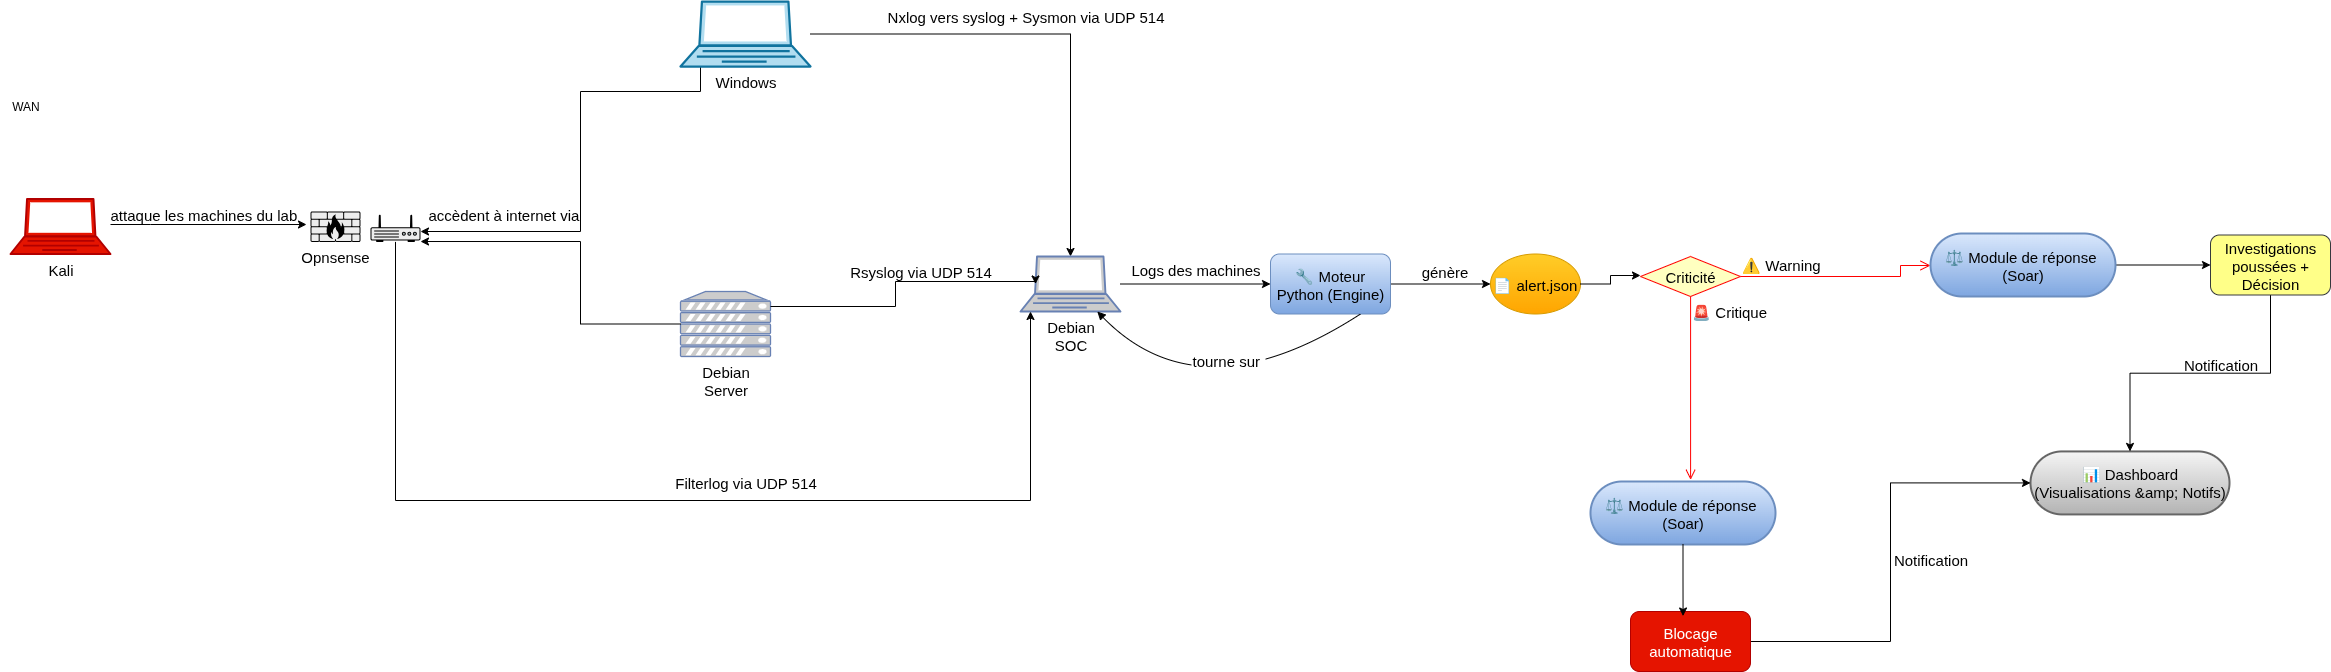
\includegraphics[width=1.05\linewidth]{Architecture.png}
    \caption{Architecture finale du projet}
    \label{fig:placeholder}
\end{figure}

\subsection{Inventaire des machines virtuelles}

\begin{table}[H]
\centering
\caption{Inventaire des machines virtuelles du laboratoire}
\label{tab:vms}
\begin{tabularx}{\textwidth}{lXllll}
\toprule
\textbf{VM} & \textbf{OS} & \textbf{RAM} & \textbf{Disque}
            & \textbf{IP LAN} & \textbf{Rôle PME} \\
\midrule
OPNsense     & FreeBSD 26.x  & 1~Go  & 8~Go  & 10.0.1.1  & Routeur/pare-feu \\
SOC          & Debian 12     & 2~Go  & 20~Go & 10.0.1.10 & Serveur de supervision \\
Debian Server& Debian 12     & 2~Go  & 15~Go & 10.0.1.20 & Serveur de fichiers/AD \\
Windows 10   & Windows 10    & 3~Go  & 40~Go & 10.0.1.30 & Poste employé \\
Kali         & Docker (hôte) &      & —     & 10.0.1.50 & Attaquant simulé \\
\midrule
\textbf{Total} & & \textbf{8~Go} & \textbf{83~Go} & & \\
\bottomrule
\end{tabularx}
\end{table}

La marge disponible de 8~Go sur 16~Go couvre l'environnement hôte
(VS~Code, virt-manager, Wireshark) avec une réserve confortable.

% ============================================================
\section{Justification des choix par composant}
% ============================================================

\subsection{Hyperviseur : KVM/QEMU + libvirt}

KVM est intégré au noyau Linux depuis la version 2.6.20 (2007).
Contrairement à VirtualBox, il ne repose sur aucun module noyau tiers
(DKMS) et ne nécessite aucune recompilation lors des mises à jour du
noyau hôte \cite{kvm_kernel}. Sur Fedora~44 avec un noyau récent (7.0.12),
cette stabilité est critique pour un projet dont la durée dépasse dix semaines.

libvirt fournit une API unifiée pour la gestion des VMs, des réseaux virtuels
et des snapshots. vagrant-libvirt permet d'intégrer Vagrant dans cet
écosystème sans sortir du provider KVM.

\subsection{Pare-feu : OPNsense}

\begin{table}[H]
\centering
\caption{Comparaison des solutions de pare-feu pour le laboratoire}
\label{tab:firewall}
\begin{tabularx}{\textwidth}{lXXX}
\toprule
\textbf{Critère} & \textbf{OPNsense} & \textbf{pfSense} & \textbf{Alpine Linux} \\
\midrule
Licence          & BSD libre         & Netgate (restrictions depuis 2023) & MIT \\
Interface web    & Oui, native       & Oui, native       & Non (scripts manuels) \\
Export syslog    & Natif GUI         & Natif GUI         & Configuration manuelle \\
API REST         & Oui (OPNsense API)& Limitée           & Non \\
Logs filterlog   & Oui               & Oui               & Non standard \\
Réalisme PME     & Élevé             & Élevé             & Faible \\
\bottomrule
\end{tabularx}
\end{table}

OPNsense est retenu pour trois raisons. Premièrement, son interface web
permet de configurer l'export syslog sans écriture de scripts, ce qui réduit
la complexité d'infrastructure. Deuxièmement, son API REST est utilisée par
le module de réponse automatisée pour injecter des règles de blocage dynamiques.
Troisièmement, pfSense a introduit des restrictions de redistribution depuis
son rachat par Netgate en 2023, ce qui le rend inadapté à un projet académique
open source \cite{pfsense_netgate}.

\subsection{Système d'exploitation des serveurs Linux : Debian 12}

Debian est retenu à la place d'Ubuntu Server pour l'ensemble des VMs Linux
(SOC et Debian Server). Debian suit une philosophie minimaliste~: aucun service
superflu n'est installé par défaut, ce qui réduit le bruit dans les logs système
et rend les mesures de performance plus précises. Python~3.12, rsyslog, Samba~4
et Apache~2 sont disponibles dans les dépôts officiels sans nécessiter de PPA ( Personal Package Archive )
additionnels \cite{debian_stable}.

L'homogénéité du système d'exploitation entre les deux serveurs Linux simplifie
également la maintenance et la reproductibilité du laboratoire.

\subsection{Debian Server : Samba 4 AD + Apache + Dolibarr}

\subsubsection{Samba 4 en mode Active Directory Domain Controller}

Les PME togolaises qui centralisent l'authentification de leurs postes de travail
utilisent soit Windows Server AD (coût de licence prohibitif), soit Samba~4 en
mode DC, qui implémente le protocole Kerberos et LDAP (Lightweight Directory Access Protocol) de manière compatible avec
Active Directory \cite{samba4_ad}. Samba~4 AD permet à Windows~10 de rejoindre
le domaine, ce qui génère des Event IDs Kerberos (4768, 4769) corrélables avec
les accès aux partages SMB côté serveur.

Les partages de fichiers simulés représentent les données sensibles d'une PME~:
documents de direction, relevés Mobile Money, fichiers comptables. Ces données
sont la cible du scénario d'exfiltration S2.

La RAM allouée à Debian Server est portée à 2~Go pour absorber le chargement
des processus Samba~4 AD (smbd, nmbd, winbindd, samba-ad-dc) et du serveur web
simultanément.

\subsubsection{Apache + Dolibarr}

Dolibarr est l'ERP open source le plus déployé dans les PME d'Afrique
francophone~: facturation, gestion commerciale, documents internes \cite{dolibarr}.
Son déploiement sur Apache dans le laboratoire reproduit fidèlement
l'infrastructure applicative d'une PME togolaise disposant d'un budget logiciel
limité. Les logs d'accès Apache (\texttt{/var/log/apache2/access.log}) constituent
une source supplémentaire pour les scénarios d'attaque ciblant l'application web.

\subsection{Windows 10}

\subsubsection{Choix de la version}

Windows~10 est retenu plutôt que Windows~11 pour trois raisons~:
consommation mémoire inférieure (Windows~11 consomme environ 500~Mo de plus
au repos), absence d'exigences matérielles restrictives (TPM~2.0, Secure Boot)
qui compliquent la virtualisation KVM, et représentativité du parc informatique
des PME togolaises où Windows~10 reste majoritaire \cite{statcounter_africa}.

\subsubsection{Allocation mémoire}

3~Go sont alloués à Windows~10. Cette valeur tient compte de la
consommation au repos (environ 1,8--2,2~Go selon les processus background~:
Windows Update, Defender, télémétrie), du driver kernel Sysmon actif en
permanence, et de NXLog Community Edition pour le transfert des logs.
Une allocation de 2~Go provoquerait un swap constant qui fausserait
les métriques de détection.

\subsection{Collecte des logs Windows}
La stack retenue pour la collecte des logs de Windows est la combinaison \textbf{NXLog + Sysmon}.

\subsubsection{NXLog Community Edition}
\begin{table}[H]
\centering
\caption{Comparaison des agents de collecte de logs Windows}
\label{tab:nxlog}
\begin{tabularx}{\textwidth}{lXXX}
\toprule
\textbf{Critère} & \textbf{NXLog CE} & \textbf{Winlogbeat} & \textbf{Elastic Agent} \\
\midrule
Output UDP syslog & Natif (\texttt{om\_udp}) & Non natif & Non natif \\
Dépendance stack  & Aucune          & ELK Stack requis  & ELK Stack requis \\
Configuration     & Blocs input/output& YAML simple      & YAML + Fleet \\
Windows legacy    & XP → 11         & 7+ (partiel)      & 10+ \\
Poids             & Léger           & Léger             & Lourd \\
Licence           & CE gratuite     & Apache 2.0        & Elastic (restrictions) \\
\bottomrule
\end{tabularx}
\end{table}

NXLog Community Edition est retenu parce que le pipeline de collecte
cible rsyslog UDP~514 sur le SOC, pas Elasticsearch. Winlogbeat et Elastic Agent
sont conçus nativement pour la stack ELK~; les faire parler UDP syslog est
non documenté et contre-nature. NXLog dispose d'un module \texttt{om\_udp}
natif et est le standard industriel pour la collecte de logs Windows
vers des SIEM non-ELK \cite{nxlog_docs}.

\subsubsection{Sysmon}

Sysmon (System Monitor) est un service Microsoft Sysinternals qui enrichit
la journalisation Windows en capturant des événements de bas niveau~:
création de processus (Event ID~1), connexions réseau (Event ID~3),
création de fichiers (Event ID~11), entre autres \cite{sysmon_docs}.
Les Event IDs natifs Windows (4624 logon réussi, 4625 échec de logon,
4688 création de processus) ne fournissent pas le hash du processus ni
le chemin complet de l'exécutable — informations essentielles pour la
détection de fichiers malveillants via YARA.

La configuration Sysmon retenue s'inspire de la référence communautaire
SwiftOnSecurity \cite{swifton}, filtrée pour ne conserver que les Event IDs
pertinents pour les scénarios S1, S2 et S3~: 1, 3, 11 (Sysmon) et
4624, 4625, 4768, 4769 (Windows natif).

\subsection{Attaquant simulé : Kali Linux en conteneur Docker}

L'attaquant simulé (Kali Linux) est déployé en conteneur Docker sur la machine
hôte Fedora plutôt qu'en machine virtuelle dédiée. Cette approche est
justifiée par le rôle fonctionnel de Kali dans le laboratoire~: lancer des
attaques scriptées et déterministes, pas simuler un poste de travail persistant.

Les avantages sont substantiels~: économie d'environ 1~Go de RAM libérée pour
les autres VMs, caractère éphémère (le conteneur est détruit après chaque
scénario d'attaque, ce qui évite toute persistance d'état non désirée),
et disponibilité d'une image officielle \texttt{kalilinux/kali-rolling}
maintenue par Offensive Security \cite{kali_docker}.

L'accès au réseau \texttt{10.0.1.0/24} est assuré par un réseau Docker
macvlan connecté au bridge libvirt \texttt{isolated}, ce qui attribue
à Kali l'adresse \texttt{10.0.1.50} directement visible des autres VMs
et d'OPNsense.

\textbf{Justification du placement dans le LAN.} Forcer l'attaquant
à entrer par le WAN d'OPNsense ajouterait une complexité de configuration
(NAT, port forwarding, règles entrantes) sans valeur ajoutée pour les
hypothèses de recherche. Ce projet valide un moteur de \textit{corrélation}
d'événements, pas la robustesse d'un pare-feu face à des attaques externes.
Le placement de Kali dans le LAN simule un vecteur réaliste et documenté~:
menace interne ou accès VPN compromis, que le rapport INTERPOL 2025 identifie
comme prépondérant dans les incidents africains \cite{interpol2025}.

\subsection{Synchronisation temporelle : Chrony}

La précision temporelle est critique pour le moteur de corrélation~: une
dérive de 5~secondes sur une fenêtre de corrélation de 60~secondes représente
8\% d'erreur et peut provoquer des faux négatifs. Chrony est retenu à la place
du client NTP traditionnel (\texttt{ntpd}) pour sa capacité à converger
rapidement même après un redémarrage et à maintenir une précision submilliseconde
dans un environnement virtualisé \cite{chrony_docs}.

Chrony est installé sur toutes les VMs Linux. Sur Windows~10, la
synchronisation NTP est assurée par le service \texttt{W32tm} configuré
pour pointer vers \texttt{10.0.1.1} (OPNsense, qui synchronise lui-même
via son service NTP intégré).

\subsection{Transport syslog : UDP}

Le protocole UDP est retenu pour le transport syslog entre toutes les sources
et le SOC. Dans un réseau isolé de laboratoire avec peu de sources simultanées,
la garantie de livraison apportée par TCP n'est pas nécessaire. UDP élimine
tout overhead de connexion et ne peut pas bloquer rsyslog si le SOC est
momentanément saturé~; TCP introduirait un risque de back-pressure qui
perturberait la collecte pendant les pics d'événements (notamment lors des
scénarios de brute-force SSH) \cite{rsyslog_udp}.

% ============================================================
\section{Pipeline de collecte des logs}
% ============================================================

\subsection{Sources et formats}

\begin{table}[H]
\centering
\caption{Sources de logs, formats et événements collectés}
\label{tab:sources}
\begin{tabularx}{\textwidth}{lllX}
\toprule
\textbf{Source} & \textbf{Format} & \textbf{Transport} & \textbf{Événements clés} \\
\midrule
Debian Server   & syslog RFC 5424 & rsyslog UDP 514
  & \texttt{auth/authpriv} (SSH, PAM, sudo),
    \texttt{daemon} (Samba accès/échecs) \\
Windows 10      & XML EventLog + Sysmon & NXLog → UDP 514
  & 4624/4625 (logon), 4688 (process), 4663 (file access),
    Sysmon 1/3/11 \\
OPNsense        & filterlog BSD   & syslog UDP 514
  & Trafic filtré, scans réseau, connexions bloquées \\
Apache (Dolibarr)& Combined Log Format & rsyslog UDP 514
  & Requêtes HTTP, codes d'erreur, IP source \\
\bottomrule
\end{tabularx}
\end{table}

\subsection{Réception sur le SOC}

Tous les flux convergent vers rsyslog sur le SOC (port UDP~514).
rsyslog écrit les événements dans \texttt{/var/log/remote/} en séparant
les fichiers par hostname source~:

\begin{itemize}
    \item \texttt{/var/log/remote/debian.log} — Debian Server
    \item \texttt{/var/log/remote/OPNsense.internal.log} — OPNsense
    \item \texttt{/var/log/remote/DESKTOP-PME.log} — Windows 10
\end{itemize}

Le moteur Python surveille ce répertoire via \texttt{watchdog} (inotify)
et traite les nouvelles lignes en temps réel.

% ============================================================
\section{Scénarios d'attaque}
% ============================================================

Les scénarios sont ancrés dans les menaces documentées par INTERPOL~2025
pour l'Afrique de l'Ouest \cite{interpol2025}.

\begin{table}[H]
\centering
\caption{Scénarios d'attaque simulés}
\label{tab:scenarios}
\begin{tabularx}{\textwidth}{llXX}
\toprule
\textbf{ID} & \textbf{Contexte PME} & \textbf{Chaîne d'attaque} & \textbf{Sources corrélées} \\
\midrule
S1 & Brute-force SSH
   & Kali → hydra → tentatives SSH répétées sur Debian Server
   & filterlog (scan) + auth (échecs SSH) \\
S2 & Exfiltration données financières
   & Kali → nmap → brute-force SMB (CrackMapExec) → smbclient get relevés
   & filterlog + daemon (Samba) + auth \\
S3 & Compromission poste employé (BEC)
   & Kali → upload payload via partage Samba → exécution Windows → YARA match
   & Sysmon 1/11 + YARA + daemon \\
\bottomrule
\end{tabularx}
\end{table}

% ============================================================
\section{Récapitulatif des décisions architecturales}
% ============================================================

\begin{table}[H]
\centering
\caption{Récapitulatif des décisions et justifications}
\label{tab:decisions}
\begin{tabularx}{\textwidth}{lXX}
\toprule
\textbf{Composant} & \textbf{Choix retenu} & \textbf{Raison principale} \\
\midrule
Hyperviseur      & KVM/QEMU + libvirt    & Intégré au noyau, stable sans DKMS \\
Pare-feu         & OPNsense              & API REST, syslog natif, libre \\
OS serveurs      & Debian 12             & Minimalisme, homogénéité, logs propres \\
Serveur fichiers & Samba 4 AD            & Compatible AD, réalisme PME, gratuit \\
Application web  & Apache + Dolibarr     & ERP dominant Afrique francophone \\
Poste client     & Windows 10 + Sysmon   & Réalisme PME, Event IDs enrichis \\
Collecte Windows & NXLog CE              & Output UDP natif, indépendant de ELK \\
Attaquant        & Kali Docker (hôte)    & Éphémère, économie RAM, image officielle \\
NTP              & Chrony (Linux), W32tm (Windows) & Convergence rapide, précision sub-ms \\
Transport syslog & UDP                   & Pas de back-pressure, standard historique \\
\bottomrule
\end{tabularx}
\end{table}

% ============================================================
\begin{thebibliography}{99}

\bibitem{ancy_strategie}
Agence Nationale de la Cybersécurité du Togo,
\textit{Stratégie nationale de cybersécurité 2024--2028},
ANCy, Lomé, Togo, 2024.
[En ligne]. Disponible sur :
\url{https://ancy.gouv.tg/publication-de-la-strategie-nationale-de-cybersecurite-pour-le-togo/}

\bibitem{interpol2025}
INTERPOL,
\textit{Africa Cyberthreat Assessment 2025},
INTERPOL, Lyon, 2025.
[En ligne]. Disponible sur :
\url{https://www.interpol.int/content/download/21864/file/Africa\%20Cyberthreat\%20Assessment\%20Report_2025.pdf}

\bibitem{kvm_kernel}
R.~Avi Kivity \textit{et al.},
``kvm: the Linux virtual machine monitor,''
in \textit{Proceedings of the Linux Symposium}, vol.~1, 2007, pp.~225--230.

\bibitem{pfsense_netgate}
Netgate,
\textit{pfSense Plus Software — Licensing},
Netgate, 2023.
[En ligne]. Disponible sur : \url{https://www.netgate.com/pfsense-plus-software}

\bibitem{debian_stable}
The Debian Project,
\textit{Debian GNU/Linux 12 (bookworm) — Release Notes},
Debian, 2023.
[En ligne]. Disponible sur : \url{https://www.debian.org/releases/stable/}

\bibitem{samba4_ad}
The Samba Team,
\textit{Setting up Samba as an Active Directory Domain Controller},
Samba Wiki, 2024.
[En ligne]. Disponible sur :
\url{https://wiki.samba.org/index.php/Setting_up_Samba_as_an_Active_Directory_Domain_Controller}

\bibitem{dolibarr}
Dolibarr ERP/CRM,
\textit{Dolibarr — Présentation générale},
2024.
[En ligne]. Disponible sur : \url{https://www.dolibarr.org/}

\bibitem{statcounter_africa}
StatCounter,
\textit{Desktop Windows Version Market Share Africa},
StatCounter Global Stats, juin 2025.
[En ligne]. Disponible sur :
\url{https://gs.statcounter.com/windows-version-market-share/desktop/africa}

\bibitem{sysmon_docs}
Microsoft,
\textit{Sysmon — Sysinternals},
Microsoft Learn, 2024.
[En ligne]. Disponible sur :
\url{https://learn.microsoft.com/en-us/sysinternals/downloads/sysmon}

\bibitem{swifton}
SwiftOnSecurity,
\textit{sysmon-config — A Sysmon configuration file for everybody to deploy},
GitHub, 2024.
[En ligne]. Disponible sur :
\url{https://github.com/SwiftOnSecurity/sysmon-config}

\bibitem{nxlog_docs}
NXLog Ltd.,
\textit{NXLog Community Edition Reference Manual},
NXLog, 2024.
[En ligne]. Disponible sur : \url{https://docs.nxlog.co/ce/current/}

\bibitem{kali_docker}
Offensive Security,
\textit{Kali Linux Docker Image},
Docker Hub, 2024.
[En ligne]. Disponible sur : \url{https://hub.docker.com/r/kalilinux/kali-rolling}

\bibitem{chrony_docs}
R.~Curnow,
\textit{chrony — a versatile implementation of the Network Time Protocol},
chrony.tuxfamily.org, 2024.
[En ligne]. Disponible sur : \url{https://chrony-project.org/documentation.html}

\bibitem{rsyslog_udp}
Rainer Gerhards,
\textit{rsyslog Documentation — imudp: UDP Syslog Input Module},
rsyslog.com, 2024.
[En ligne]. Disponible sur : \url{https://www.rsyslog.com/doc/configuration/modules/imudp.html}

\end{thebibliography}

\end{document}